\documentclass{standalone}
\usepackage{tikz}
\usetikzlibrary{patterns, positioning}
\usepackage[sfdefault]{ClearSans} %% option 'sfdefault' activates Clear Sans as the default text font
\usepackage[T1]{fontenc}

\begin{document}
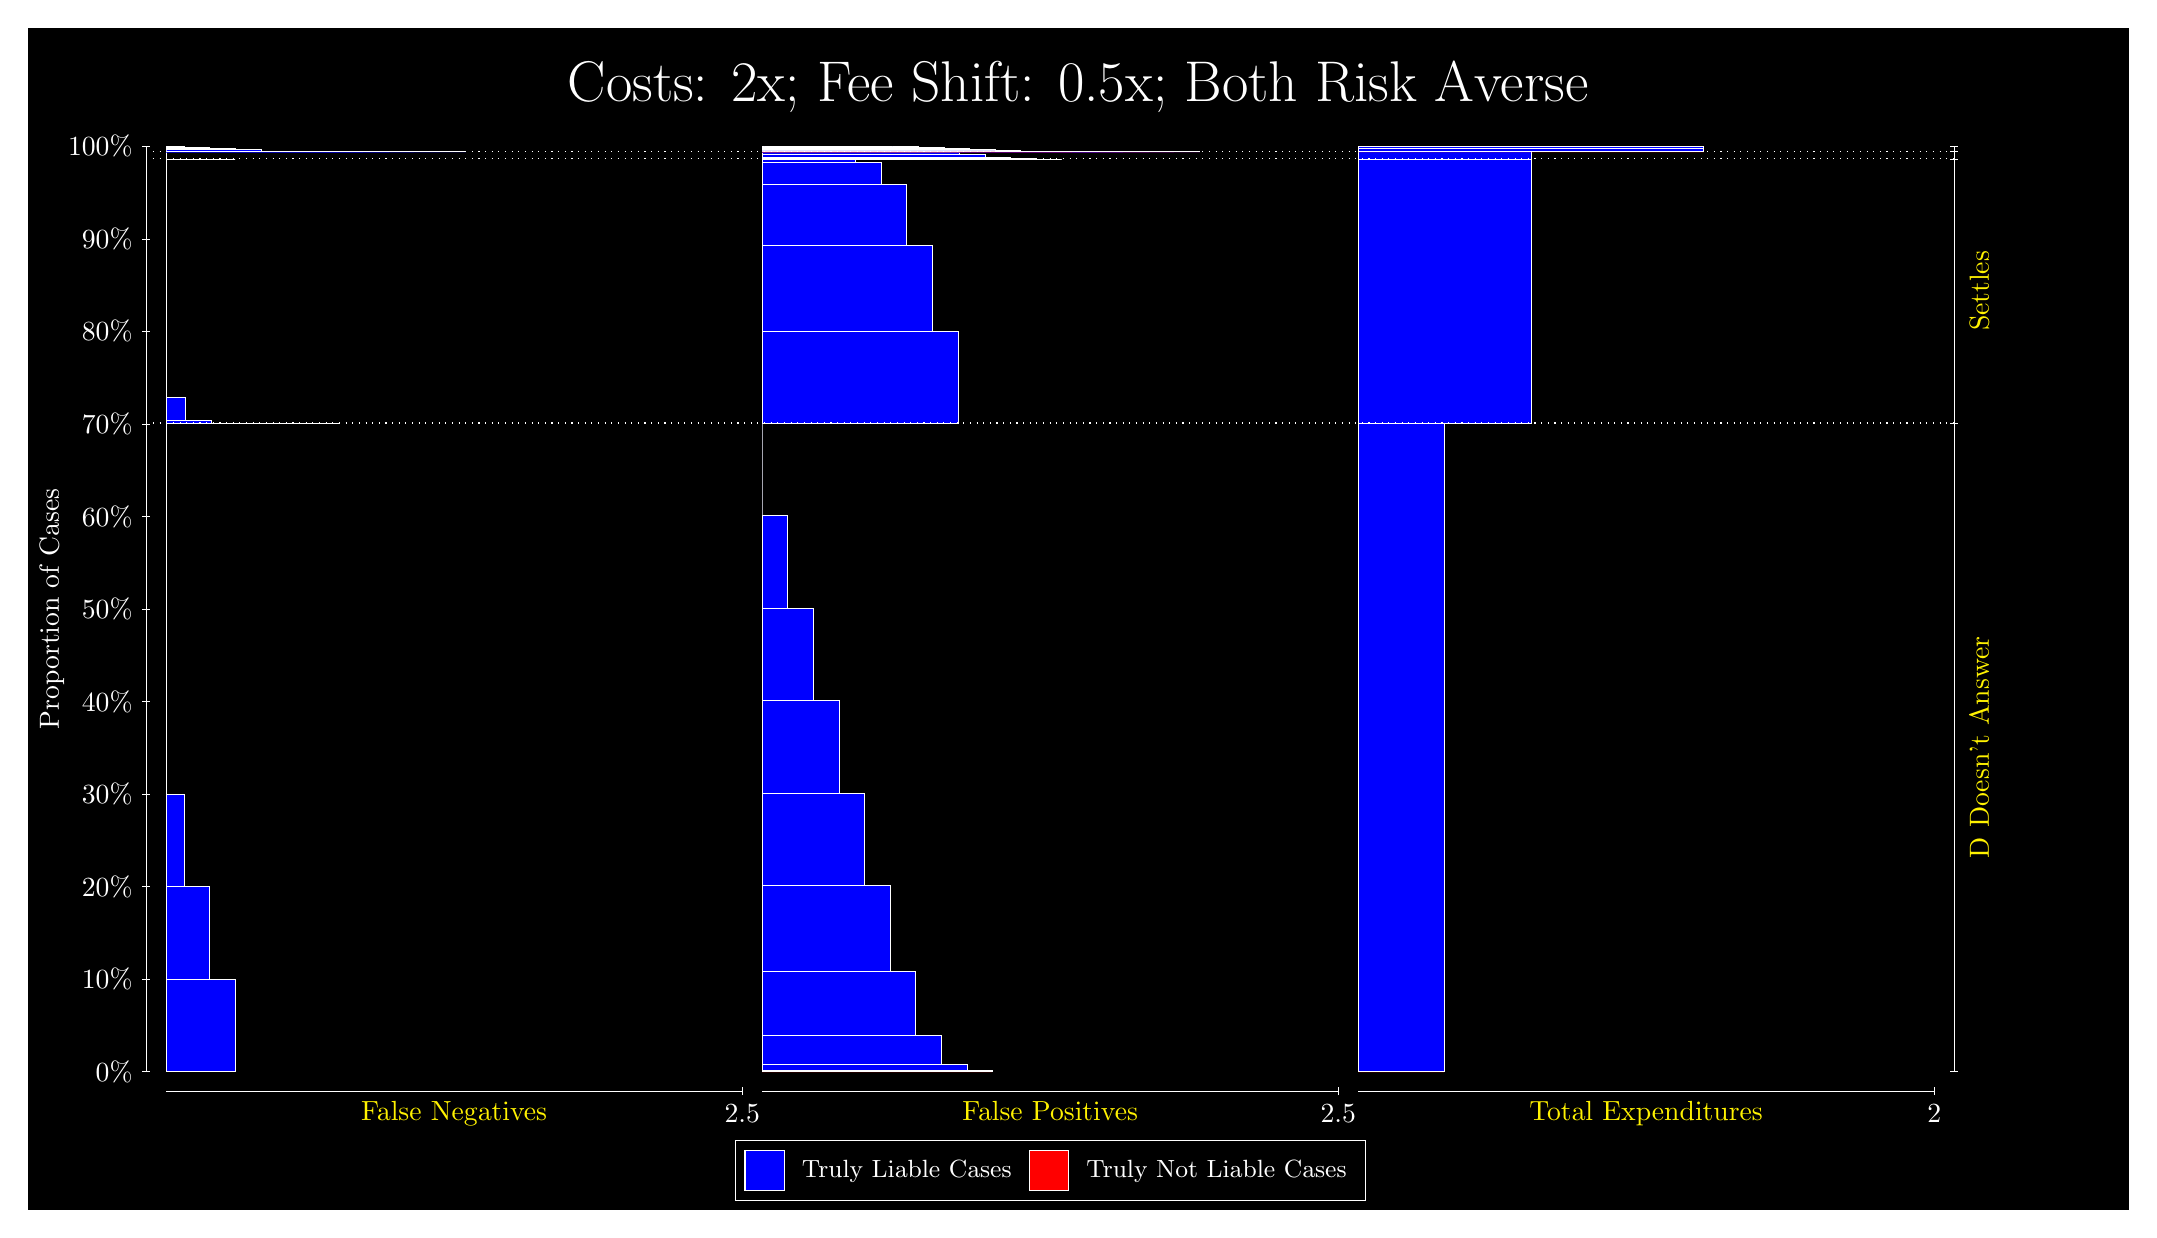
\begin{tikzpicture}
\draw[fill=black] (0,0) rectangle (26.667,15);
\draw[text=white] (0,13.5) rectangle (26.667,15) node[midway] {\huge Costs: 2x; Fee Shift: 0.5x; Both Risk Averse};
\draw[white, very thin] (1.5,1.75) -- (1.5,13.5);
\node[rotate=90, text=white, anchor=center] at (0.3, 7.625) {Proportion of Cases};
\draw[white, very thin] (1.45,1.75) -- (1.55,1.75);
\node[text=white, anchor=east] at (1.45, 1.75) {0\%};
\draw[white, very thin] (1.45,2.925) -- (1.55,2.925);
\node[text=white, anchor=east] at (1.45, 2.925) {10\%};
\draw[white, very thin] (1.45,4.1) -- (1.55,4.1);
\node[text=white, anchor=east] at (1.45, 4.1) {20\%};
\draw[white, very thin] (1.45,5.275) -- (1.55,5.275);
\node[text=white, anchor=east] at (1.45, 5.275) {30\%};
\draw[white, very thin] (1.45,6.45) -- (1.55,6.45);
\node[text=white, anchor=east] at (1.45, 6.45) {40\%};
\draw[white, very thin] (1.45,7.625) -- (1.55,7.625);
\node[text=white, anchor=east] at (1.45, 7.625) {50\%};
\draw[white, very thin] (1.45,8.8) -- (1.55,8.8);
\node[text=white, anchor=east] at (1.45, 8.8) {60\%};
\draw[white, very thin] (1.45,9.975) -- (1.55,9.975);
\node[text=white, anchor=east] at (1.45, 9.975) {70\%};
\draw[white, very thin] (1.45,11.15) -- (1.55,11.15);
\node[text=white, anchor=east] at (1.45, 11.15) {80\%};
\draw[white, very thin] (1.45,12.325) -- (1.55,12.325);
\node[text=white, anchor=east] at (1.45, 12.325) {90\%};
\draw[white, very thin] (1.45,13.5) -- (1.55,13.5);
\node[text=white, anchor=east] at (1.45, 13.5) {100\%};

\draw[white, very thin] (24.457,1.75) -- (24.457,13.5);
\draw[white, very thin] (24.407,1.75) -- (24.507,1.75);
\node[anchor=west] at (24.407, 1.75) {};
\draw[white, very thin] (24.407,9.9861) -- (24.507,9.9861);
\node[anchor=west] at (24.407, 9.9861) {};
\draw[white, very thin] (24.407,13.341) -- (24.507,13.341);
\node[anchor=west] at (24.407, 13.341) {};
\draw[white, very thin] (24.407,13.434) -- (24.507,13.434);
\node[anchor=west] at (24.407, 13.434) {};
\draw[white, very thin] (24.407,13.5) -- (24.507,13.5);
\node[anchor=west] at (24.407, 13.5) {};

\draw[white, very thin, fill=blue] (1.75,1.75) rectangle (2.6283,2.925);
\draw[white, very thin, fill=blue] (1.75,2.925) rectangle (2.303,4.1);
\draw[white, very thin, fill=blue] (1.75,4.1) rectangle (1.9777,5.275);
\draw[white, very thin, fill=red] (1.75,5.275) rectangle (1.75,5.275);
\draw[white, very thin, fill=blue] (1.75,5.275) rectangle (1.75,9.9861);
\draw[white, very thin, fill=blue] (1.75,9.9861) rectangle (3.9457,9.9861);
\draw[white, very thin, fill=blue] (1.75,9.9861) rectangle (3.6204,9.9861);
\draw[white, very thin, fill=blue] (1.75,9.9861) rectangle (3.2951,9.9861);
\draw[white, very thin, fill=blue] (1.75,9.9861) rectangle (2.9698,9.9861);
\draw[white, very thin, fill=blue] (1.75,9.9861) rectangle (2.6445,9.9873);
\draw[white, very thin, fill=blue] (1.75,9.9873) rectangle (2.3192,10.025);
\draw[white, very thin, fill=blue] (1.75,10.025) rectangle (1.994,10.313);
\draw[white, very thin, fill=red] (1.75,10.313) rectangle (1.75,10.313);
\draw[white, very thin, fill=blue] (1.75,10.313) rectangle (1.75,13.341);
\draw[white, very thin, fill=blue] (1.75,13.341) rectangle (2.6283,13.341);
\draw[white, very thin, fill=blue] (1.75,13.341) rectangle (2.303,13.341);
\draw[white, very thin, fill=blue] (1.75,13.341) rectangle (1.9777,13.341);
\draw[white, very thin, fill=red] (1.75,13.341) rectangle (1.75,13.341);
\draw[white, very thin, fill=blue] (1.75,13.341) rectangle (1.75,13.434);
\draw[white, very thin, fill=blue] (1.75,13.434) rectangle (5.5558,13.434);
\draw[white, very thin, fill=blue] (1.75,13.434) rectangle (5.2305,13.434);
\draw[white, very thin, fill=blue] (1.75,13.434) rectangle (4.9052,13.434);
\draw[white, very thin, fill=blue] (1.75,13.434) rectangle (4.58,13.434);
\draw[white, very thin, fill=blue] (1.75,13.434) rectangle (4.58,13.434);
\draw[white, very thin, fill=blue] (1.75,13.434) rectangle (4.2547,13.434);
\draw[white, very thin, fill=blue] (1.75,13.434) rectangle (4.2547,13.434);
\draw[white, very thin, fill=blue] (1.75,13.434) rectangle (3.9294,13.434);
\draw[white, very thin, fill=blue] (1.75,13.434) rectangle (3.6041,13.436);
\draw[white, very thin, fill=blue] (1.75,13.436) rectangle (3.2788,13.436);
\draw[white, very thin, fill=blue] (1.75,13.436) rectangle (3.2788,13.443);
\draw[white, very thin, fill=blue] (1.75,13.443) rectangle (2.9535,13.443);
\draw[white, very thin, fill=blue] (1.75,13.443) rectangle (2.9535,13.443);
\draw[white, very thin, fill=blue] (1.75,13.443) rectangle (2.9535,13.457);
\draw[white, very thin, fill=blue] (1.75,13.457) rectangle (2.9535,13.457);
\draw[white, very thin, fill=blue] (1.75,13.457) rectangle (2.6283,13.457);
\draw[white, very thin, fill=blue] (1.75,13.457) rectangle (2.6283,13.475);
\draw[white, very thin, fill=blue] (1.75,13.475) rectangle (2.303,13.475);
\draw[white, very thin, fill=blue] (1.75,13.475) rectangle (2.303,13.475);
\draw[white, very thin, fill=blue] (1.75,13.475) rectangle (2.303,13.487);
\draw[white, very thin, fill=blue] (1.75,13.487) rectangle (2.303,13.489);
\draw[white, very thin, fill=blue] (1.75,13.489) rectangle (1.9777,13.489);
\draw[white, very thin, fill=blue] (1.75,13.489) rectangle (1.9777,13.493);
\draw[white, very thin, fill=blue] (1.75,13.493) rectangle (1.9777,13.497);
\draw[white, very thin, fill=red] (1.75,13.497) rectangle (1.75,13.497);
\draw[white, very thin, fill=blue] (1.75,13.497) rectangle (1.75,13.5);
\draw[white, very thin, fill=red] (9.3189,1.75) rectangle (12.246,1.75);
\draw[white, very thin, fill=blue] (9.3189,1.75) rectangle (12.246,1.7606);
\draw[white, very thin, fill=blue] (9.3189,1.7606) rectangle (11.921,1.8447);
\draw[white, very thin, fill=blue] (9.3189,1.8447) rectangle (11.596,2.2095);
\draw[white, very thin, fill=blue] (9.3189,2.2095) rectangle (11.271,3.0221);
\draw[white, very thin, fill=blue] (9.3189,3.0221) rectangle (10.945,4.1186);
\draw[white, very thin, fill=blue] (9.3189,4.1186) rectangle (10.62,5.2863);
\draw[white, very thin, fill=blue] (9.3189,5.2863) rectangle (10.295,6.461);
\draw[white, very thin, fill=blue] (9.3189,6.461) rectangle (9.9694,7.636);
\draw[white, very thin, fill=blue] (9.3189,7.636) rectangle (9.6442,8.8111);
\draw[white, very thin, fill=blue] (9.3189,8.8111) rectangle (9.3189,9.9861);
\draw[white, very thin, fill=red] (9.3189,9.9861) rectangle (11.807,9.9861);
\draw[white, very thin, fill=blue] (9.3189,9.9861) rectangle (11.807,11.15);
\draw[white, very thin, fill=blue] (9.3189,11.15) rectangle (11.482,12.237);
\draw[white, very thin, fill=blue] (9.3189,12.237) rectangle (11.157,13.014);
\draw[white, very thin, fill=blue] (9.3189,13.014) rectangle (10.831,13.303);
\draw[white, very thin, fill=blue] (9.3189,13.303) rectangle (10.506,13.34);
\draw[white, very thin, fill=blue] (9.3189,13.34) rectangle (10.181,13.341);
\draw[white, very thin, fill=blue] (9.3189,13.341) rectangle (9.8556,13.341);
\draw[white, very thin, fill=blue] (9.3189,13.341) rectangle (9.5303,13.341);
\draw[white, very thin, fill=blue] (9.3189,13.341) rectangle (9.3189,13.341);
\draw[white, very thin, fill=red] (9.3189,13.341) rectangle (13.125,13.341);
\draw[white, very thin, fill=blue] (9.3189,13.341) rectangle (13.125,13.341);
\draw[white, very thin, fill=blue] (9.3189,13.341) rectangle (12.799,13.342);
\draw[white, very thin, fill=blue] (9.3189,13.342) rectangle (12.474,13.356);
\draw[white, very thin, fill=blue] (9.3189,13.356) rectangle (12.149,13.401);
\draw[white, very thin, fill=blue] (9.3189,13.401) rectangle (11.824,13.43);
\draw[white, very thin, fill=blue] (9.3189,13.43) rectangle (11.498,13.434);
\draw[white, very thin, fill=blue] (9.3189,13.434) rectangle (11.173,13.434);
\draw[white, very thin, fill=blue] (9.3189,13.434) rectangle (10.848,13.434);
\draw[white, very thin, fill=blue] (9.3189,13.434) rectangle (10.522,13.434);
\draw[white, very thin, fill=blue] (9.3189,13.434) rectangle (10.197,13.434);
\draw[white, very thin, fill=red] (9.3189,13.434) rectangle (14.881,13.434);
\draw[white, very thin, fill=blue] (9.3189,13.434) rectangle (14.881,13.434);
\draw[white, very thin, fill=red] (9.3189,13.434) rectangle (14.556,13.434);
\draw[white, very thin, fill=blue] (9.3189,13.434) rectangle (14.556,13.434);
\draw[white, very thin, fill=red] (9.3189,13.434) rectangle (14.231,13.434);
\draw[white, very thin, fill=blue] (9.3189,13.434) rectangle (14.231,13.434);
\draw[white, very thin, fill=blue] (9.3189,13.434) rectangle (13.905,13.434);
\draw[white, very thin, fill=red] (9.3189,13.434) rectangle (13.905,13.434);
\draw[white, very thin, fill=blue] (9.3189,13.434) rectangle (13.905,13.434);
\draw[white, very thin, fill=red] (9.3189,13.434) rectangle (13.58,13.434);
\draw[white, very thin, fill=blue] (9.3189,13.434) rectangle (13.58,13.434);
\draw[white, very thin, fill=blue] (9.3189,13.434) rectangle (13.58,13.434);
\draw[white, very thin, fill=red] (9.3189,13.434) rectangle (13.255,13.434);
\draw[white, very thin, fill=blue] (9.3189,13.434) rectangle (13.255,13.435);
\draw[white, very thin, fill=blue] (9.3189,13.435) rectangle (13.255,13.435);
\draw[white, very thin, fill=blue] (9.3189,13.435) rectangle (12.93,13.436);
\draw[white, very thin, fill=red] (9.3189,13.436) rectangle (12.93,13.436);
\draw[white, very thin, fill=blue] (9.3189,13.436) rectangle (12.93,13.437);
\draw[white, very thin, fill=red] (9.3189,13.437) rectangle (12.604,13.437);
\draw[white, very thin, fill=blue] (9.3189,13.437) rectangle (12.604,13.443);
\draw[white, very thin, fill=blue] (9.3189,13.443) rectangle (12.604,13.445);
\draw[white, very thin, fill=red] (9.3189,13.445) rectangle (12.279,13.445);
\draw[white, very thin, fill=blue] (9.3189,13.445) rectangle (12.279,13.459);
\draw[white, very thin, fill=blue] (9.3189,13.459) rectangle (12.279,13.459);
\draw[white, very thin, fill=blue] (9.3189,13.459) rectangle (11.954,13.464);
\draw[white, very thin, fill=red] (9.3189,13.464) rectangle (11.954,13.464);
\draw[white, very thin, fill=blue] (9.3189,13.464) rectangle (11.954,13.477);
\draw[white, very thin, fill=blue] (9.3189,13.477) rectangle (11.954,13.477);
\draw[white, very thin, fill=blue] (9.3189,13.477) rectangle (11.628,13.483);
\draw[white, very thin, fill=blue] (9.3189,13.483) rectangle (11.628,13.487);
\draw[white, very thin, fill=blue] (9.3189,13.487) rectangle (11.628,13.491);
\draw[white, very thin, fill=blue] (9.3189,13.491) rectangle (11.628,13.491);
\draw[white, very thin, fill=blue] (9.3189,13.491) rectangle (11.303,13.496);
\draw[white, very thin, fill=blue] (9.3189,13.496) rectangle (11.303,13.498);
\draw[white, very thin, fill=blue] (9.3189,13.498) rectangle (11.303,13.498);
\draw[white, very thin, fill=blue] (9.3189,13.498) rectangle (10.978,13.5);
\draw[white, very thin, fill=blue] (9.3189,13.5) rectangle (10.978,13.5);
\draw[white, very thin, fill=blue] (9.3189,13.5) rectangle (10.978,13.5);
\draw[white, very thin, fill=blue] (9.3189,13.5) rectangle (10.653,13.5);
\draw[white, very thin, fill=blue] (9.3189,13.5) rectangle (10.653,13.5);
\draw[white, very thin, fill=blue] (9.3189,13.5) rectangle (10.653,13.5);
\draw[white, very thin, fill=blue] (9.3189,13.5) rectangle (10.327,13.5);
\draw[white, very thin, fill=blue] (9.3189,13.5) rectangle (10.327,13.5);
\draw[white, very thin, fill=blue] (9.3189,13.5) rectangle (10.002,13.5);
\draw[white, very thin, fill=blue] (9.3189,13.5) rectangle (10.002,13.5);
\draw[white, very thin, fill=blue] (9.3189,13.5) rectangle (10.002,13.5);
\draw[white, very thin, fill=blue] (9.3189,13.5) rectangle (9.6767,13.5);
\draw[white, very thin, fill=blue] (9.3189,13.5) rectangle (9.6767,13.5);
\draw[white, very thin, fill=blue] (9.3189,13.5) rectangle (9.3514,13.5);
\draw[white, very thin, fill=blue] (9.3189,13.5) rectangle (9.3189,13.5);
\draw[white, very thin, fill=red] (16.888,1.75) rectangle (17.986,1.75);
\draw[white, very thin, fill=blue] (16.888,1.75) rectangle (17.986,9.9861);
\draw[white, very thin, fill=red] (16.888,9.9861) rectangle (19.083,9.9861);
\draw[white, very thin, fill=blue] (16.888,9.9861) rectangle (19.083,13.341);
\draw[white, very thin, fill=red] (16.888,13.341) rectangle (19.083,13.341);
\draw[white, very thin, fill=blue] (16.888,13.341) rectangle (19.083,13.434);
\draw[white, very thin, fill=red] (16.888,13.434) rectangle (21.279,13.434);
\draw[white, very thin, fill=blue] (16.888,13.434) rectangle (21.279,13.481);
\draw[white, very thin, fill=red] (16.888,13.481) rectangle (21.279,13.481);
\draw[white, very thin, fill=blue] (16.888,13.481) rectangle (21.279,13.5);
\draw[white, dotted] (1.5,9.9861) -- (24.457,9.9861);
\draw[white, dotted] (1.5,13.341) -- (24.457,13.341);
\draw[white, dotted] (1.5,13.434) -- (24.457,13.434);
\draw[white, very thin] (1.75,1.5) -- (9.0689,1.5);
\node[text=yellow, anchor=north] at (5.4094, 1.5) {False Negatives};
\draw[white, very thin] (9.0689,1.45) -- (9.0689,1.55);
\node[text=white, anchor=north] at (9.0689, 1.45) {2.5};

\draw[white, very thin] (9.3189,1.5) -- (16.638,1.5);
\node[text=yellow, anchor=north] at (12.978, 1.5) {False Positives};
\draw[white, very thin] (16.638,1.45) -- (16.638,1.55);
\node[text=white, anchor=north] at (16.638, 1.45) {2.5};

\draw[white, very thin] (16.888,1.5) -- (24.207,1.5);
\node[text=yellow, anchor=north] at (20.547, 1.5) {Total Expenditures};
\draw[white, very thin] (24.207,1.45) -- (24.207,1.55);
\node[text=white, anchor=north] at (24.207, 1.45) {2};

\node[text=yellow, centered, rotate=90] at (24.777, 5.868) {D Doesn't Answer};
\node[text=yellow, centered, rotate=90] at (24.777, 11.664) {Settles};



\draw (12.978300999999998,1.5) node[draw=none] (baseCoordinate) {};
\begin{scope}[align=center]
        \matrix[scale=0.5, draw=white, below=0.5cm of baseCoordinate, nodes={draw}, column sep=0.1cm]{
            \node[rectangle, draw, minimum width=0.5cm, minimum height=0.5cm, fill=blue] {}; &
            \node[draw=none, font=\small, text=white] (B) {Truly Liable Cases}; &
            \node[rectangle, draw, minimum width=0.5cm, minimum height=0.5cm, fill=red] {}; &
            \node[draw=none, font=\small, text=white] (B) {Truly Not Liable Cases}; \\
            };
\end{scope}

\end{tikzpicture}
\end{document}